\chapter{Standard DASH-MPEG}
\label{cha:rozdzial4}

\section{Wprowadzenie}
Poniższy rozdział opisuje standard Dynamic Adaptive Streaming over HTTP (DASH). Po zarysie historycznym i odniesieniu do pokrewnych technologii zaprezentowany zostaje podrozdział \ref{sec:dash-arch} zawierający zwięzły opis działania systemów wspierających strumieniowanie danych multimedialnych z wykorzystaniem DASH. Kolejne podrozdziały skupiają się na wybranych aspektach i funkcjonalnościach tego standardu takich jak hierarchiczna struktura modelu danych multimedialnych, synchronizacja strumieni oraz profile.

\section{Zarys historyczny}
Dynamic Adaptive Streaming over HTTP jest adaptacyjną techniką strumieniowania danych w sieciach komputerowych. Jest to technologia spokrewniona z Microsoft Smooth Streaming~\cite{MicroS}, Adobe Systems HTTP Dynamic Streaming~\cite{ADOBES} oraz Apple Inc. HTTP Live Streaming~\cite{APPLES}.

Prace nad standardem prowadzone przez grupę MPEG rozpoczęły się w 2010 roku. W 2011 standard DASH pojawił się jako draft, a międzynarodowym standardem stał się w kwietniu 2012 dzięki publikacji ISO/IEC 23009-1:2012~\cite{ISO-IEC-DASH}. Pierwsza demonstracja na szerszą skalę systemów opartych na DASH miała miejsce podczas igrzysk w Londynie w 2012 roku. Wdrożony tam system pozwalał 1000 użytkowników na żywo śledzić wydarzenia sportowe za pomocą laptopów, smartfonów i tabletów. W lipcu 2013 wprowadzono do standardu poprawki.

Do obecnych implementacji DASH zaliczają się:
\begin{itemize}
\item DASH Player i wtyczka do VLC, które powstały na uniwerstytecie ITEC w Klagenfurt (październik~2011),
\item biblioteki libdash (open-source) oraz bitdash (rozwiązanie komercyjne) należące do austriackiej firmy bitmovin GmbH (styczeń~2013),
\item zestaw narzędzi do przetwarzania plików multimedialnych oraz zbiór odtwarzaczy (dla HTML5, Flash, Silverlight, Chromecast) należący do castLabs GmbH (marzec~2014).
\end{itemize}

\section{Systemy implementujące DASH}
W podejściu stosowanym w standardzie DASH logika strumieniowania zostaje w całości przeniesiona na aplikację klienta. Rolę serwera DASH może pełnić serwer HTTP (np. Apache lub Nginx) na którym umieszczone zostaną dane przeznaczone do strumieniowania.
\label{sec:dash-arch}

\begin{figure}[h!]
	\centering
		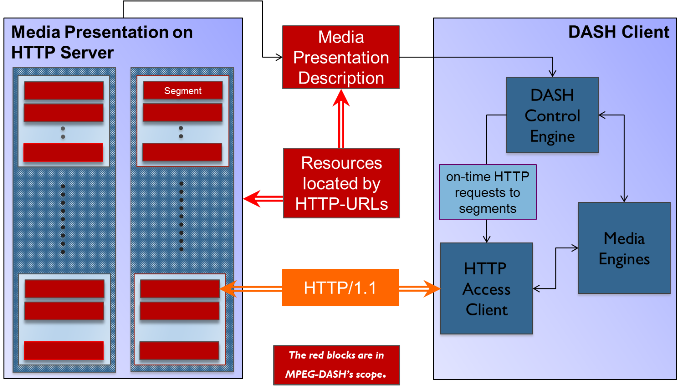
\includegraphics{dash}
	\caption{Standard MPEG-DASH i przykładowa architektura klienta DASH, źródło:~\cite{DASH}}
	\label{fig:dash}
\end{figure}

Dane multimedialne, które będą podlegały operacji strumieniowania, należy odpowiednio przygotować. Powinny one być dostępne w kilku wersjach\footnote{Akceptowalne jest przygotowanie tylko jednej wersji danych, ale uniemożliwi to operację strumieniowania adaptacyjnego.} różniących się jakością (a co za tym idzie również wielkością). Każda kopia powinna zostać podzielona na ponumerowane części (segmenty), które razem tworzą spójną całość. Na rysunku~\ref{fig:dash}~prostokąt po lewej stronie symbolizuje serwer WWW. Kopie pliku multimedialnego (niebieskie prostokąty wewnątrz serwera) składają się z segmentów (czerwone prostokąty). 

Od długości segmentów zależy szybkość przystosowywania się aplikacji DASH do zmieniających się warunków w sieci (np. przepustowości). Aplikacja klienta może dokonać przełączenia pomiędzy wersjami strumieniowanych danych tylko podczas tzw. \textit{Stream Access Points} (SAP). Są to pozycje w strumieniu danych multimedialnych, które nie wymagają informacji zawartych we wcześniejszych segmentach w celu odtwarzania późniejszych segmentów. Zwykle te pozycje znajdują się pomiędzy kolejnymi segmentami w celu uproszczenia procedur adaptacyjnych i ich implementacji. Innym częstym zabiegiem upraszczającym strumieniowanie i odtwarzanie danych jest wyrównanie czasu trwania odpowiadających sobie segmentów dla całego zbioru (\textit{Adaptation Set}) wersji danych multimedialnych (\textit{Representation})\footnote{Elementy \textit{Representation} oraz \textit{Adaptation Set} zostały szerzej opisane w podrozdziale \ref{sec:structure}.}. Powyższy przykład został zobrazowany na rysunku \ref{fig:segmentalignment}.

Przygotowane dane należy opisać za pomocą języka XML w postaci dokumentu MPD (Media Presentation Description). Plik MPD pozwala aplikacji klienta na poznanie struktury danych znajdujących się na serwerze. Zawiera adresy URL poszczególnych segmentów, czasy ich trwania, informacje na temat kodowania danych, rozdzielczości oraz minimalnych przepustowości potrzebnych do strumieniowania danych i ich odtwarzania w czasie rzeczywistym. Dokument MPD musi zostać dostarczony do aplikacji klienta, która następnie parsuje jego zawartość i rozpoczyna strumieniowanie danych. W trakcie strumieniowania, aplikacja klienta wybiera w sposób dynamiczny wersję danych i pobiera kolejne segmenty za pomocą protokołu HTTP.

\begin{figure}[h!]
	\centering
		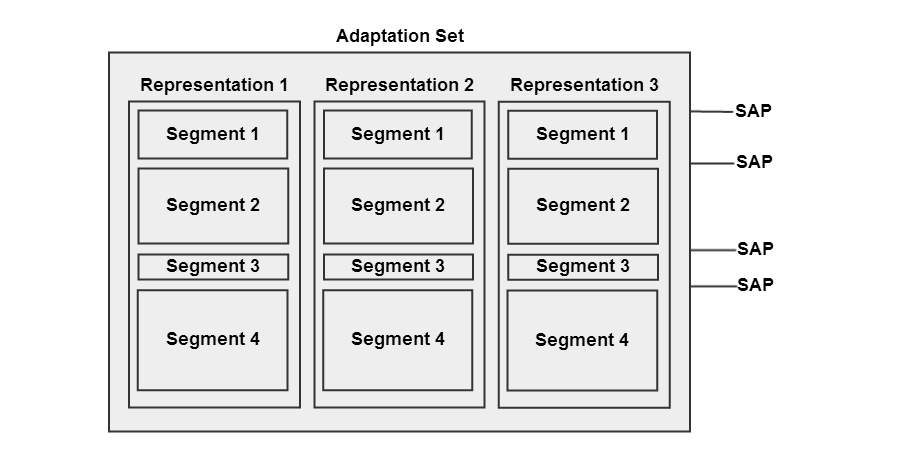
\includegraphics[width=\linewidth]{segmentalignment}
	\caption{Wizualizacja struktury danych pozwalającej na efektywne strumieniowanie adaptacyjne.}
	\label{fig:segmentalignment}
\end{figure}

Dzięki hierarchicznemu ułożeniu danych na serwerze i funkcjonalności logicznego odseparowania danych do osobnych strumieni możliwe jest dokonanie personalizacji przesyłanych danych. Przykładowo, jeżeli plik video znajdujący się na serwerze posiada kilka różnych wersji językowych napisów to możliwy jest automatyczny wybór odpowiednich napisów na podstawie preferencji klienta lub języka ustawionego na jego urządzeniu.
 
Standard DASH działa niezależnie od sposobu kodowania danych i jest łatwo implementowalny w Internecie, ponieważ jest oparty na stosie TCP/IP. Dzięki wykorzystaniu protokołu HTTP może również współpracować z istniejącą infrastrukturą w postaci filtrów, zapór, urządzeń NAT i cache~\cite{DASH}.

\section{Hierarchiczna struktura modelu danych}
\label{sec:structure}

Struktura modelu danych multimedialnych jest opisywana plikiem Media Presentation Description za pomocą języka XML i ma charakter hierarchiczny (zob.~rysunek~\ref{fig:mpd}). Lewy prostokąt symbolizuje plik MPD, który zawiera kilka elementów typu \textit{Period} (środkowy prostokąt na rysunku~\ref{fig:mpd}) oraz może zawierać informacje na temat profilu (zob.~\ref{sec:profile}). Elementy \textit{Period} reprezentują ciągłą część danych multimedialnych, które charakteryzują się takim samym zestawem parametrów. Do zestawu tych parametrów mogą należeć:
\begin{itemize}
	\item zbiór dostępnych wersji plików multimedialnych,
	\item wersje językowe dla dźwięku,
	\item wersje językowe napisów,
	\item sposób kodowania danych,
	\item itd...
\end{itemize}
Parametry te pozostają niezmienne w pojedynczym elemencie \textit{Period}, ale mogą występować różnice pomiędzy kolejnymi elementami tego typu.
Wszystkie elementy \textit{Period} posiadają znacznik czasowy pozwalający na ustalenie ich kolejności, a dane znajdujące się w kolejnych elementach tworzą ciągły strumień danych multimedialnych.

\begin{figure}
	\centering
		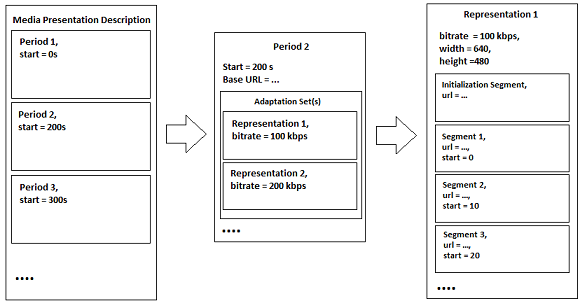
\includegraphics[width=\linewidth]{mpd}
	\caption{Struktura modelu danych, na podstawie~\cite{ISO-IEC-DASH}}
	\label{fig:mpd}
\end{figure}

Dane znajdujące się w pojedynczym elemencie \textit{Period} mogą zostać rozdzielone pomiędzy kilka elementów o nazwie \textit{Adaptation Set}. \textit{Adaptation Set} reprezentuje jedną lub kilka wersji komponentów danych multimedialnych. Przykładowo, możliwe jest odseparowanie danych video i audio poprzez przechowywanie ich w osobnych elementach \textit{Adaptation Set}. Dane tekstowe (napisy) również mogą zostać wydzielone w podobny sposób. Rezygnacja z multipleksacji danych pozwala na wprowadzenie kilku wersji danych (audio lub napisy dostępne w różnych wersjach językowych).

Każdy \textit{Adaptation Set} zawiera jeden lub kilka elementów typu \textit{Representation} (prawy prostokąt na rysunku~\ref{fig:mpd}). Dane multimedialne w ramach \textit{Representation} są wystarczające do odtworzenia pełnego i spójnego pliku multimedialnego zanim został podzielony na części (\textit{Segments}). Typowo, dane multimedialne w poszczególnych elementach \textit{Representation} różnią się jakością, co w rezultacie wpływa na ich wielkość. W trakcie strumieniowania aplikacja klienta może wybierać pomiędzy różnymi wersjami danych na podstawie warunków panujących w sieci komputerowej (dostępna przepustowość, RTT\footnote{Round Trip Time - minimalny czas potrzebny na komunikację od nadawcy do odbiorcy i z powrotem.}) lub innych czynników.

Dane multimedialne w ramach \textit{Representation} są podzielone na wiele części typu \textit{Segments}. Każdy \textit{Segment} ma określony czas trwania odpowiadający czasowi odtwarzania danych w nim zawartych oraz znacznik czasowy pozwalający na ustalenie ich właściwej kolejności. Elementy \textit{Segment} należące do tego samego \textit{Representation} zwykle mają porównywalny czas trwania. Możliwy jest dalszy podział danych w obrębie pojedynczego elementu \textit{Segment} na \textit{Subsegments}. W celu umożliwienia synchronizacji podczas odtwarzania danych wykorzystywany jest \textit{Segment index} dostarczający informacji o położeniu \textit{Subsegments} na osi czasu prezentacji (zob. \ref{subsec:presentationtimeline}). \textit{Segment index} ma znaczenie lokalne w obrębie pojedynczego elementu \textit{Segment}. Aplikacja klienta ma możliwość pobrania \textit{Segment index} i następnie wysłania zapytań HTTP dotyczących jedynie wybranych \textit{Subsegments}.

\section{DASH timelines}

Standard DASH definiuje dwie osie czasu. Pierwsza z nich, opisana w sekcji \ref{subsec:presentationtimeline} stanowi główny komponent standardu odpowiadający za synchronizację pobieranych danych multimedialnych. \textit{Segment availability timeline} pozwala na sprawne zarządzanie dostępnością segmentów potrzać transmisji w czasie rzeczywistym.

\subsection{Media presentation timeline}
\label{subsec:presentationtimeline}

Pierwsza z dwóch osi czasu pozwala na synchronizację odtwarzania komponentów danych multimedialnych (audio/video/text). Metadane wymagane do synchronizacji można uzyskać z pliku MPD. Elementy \textit{Period} oraz \textit{Segment} posiadają atrybut \textit{start} (zob. rysunek~\ref{fig:mpd}) pozwalający na określenie czasu w którym należy rozpocząć odtwarzanie zawieranych przez nie danych. W celu obliczenia bezwzględnego czasu w którym należy odtworzyć dany \textit{Segment} należy obliczyć sumę składającą się z wartości atrybutu \textit{start} elemntu \textit{Period} do którego dany \textit{Segment} należy oraz wartości atrybutu \textit{start} dla danego elementu typu \textit{Segment}.

\subsection{Segment availability timeline}

Druga z osi czasu jest wykorzystywana do wskazywania aplikacji klienta okien czasowych w jakich dostępne są dane multimedialne. Okna te nazywane są \textit{Segment Availability Times}. Aplikacja klienta powinna sprawdzić dostępność danych (reprezentowanych przez \textit{Segment} posiadający własny URL) przed próbą ich pobrania. W przypadku modelów ``On Demand'' takich jak VoD\footnote{Video On Demand - usługa pozwalająca na odtwarzanie danych multimedialnych w wybranym przez użytkownika czasie, późniejszym niż czas emisji.} plik MPD nie ulega zmianie i okna czasowe dla wszystkich danych multimedialnych są jednakowe. Takie podejście pozwala klientowi na odtwarzanie danych znajdujących się w dowolnym miejscu na osi czasowej (możliwość wprowadzenia powtórek, przewijana transmisji do przodu lub do tyłu). Dla usług ``na żywo'', gdzie plik MPD jest aktualizowany w czasie działania aplikacji klienckich, okna czasowe charakteryzują się ograniczonym czasem życia związanym z położeniem danych multimedialnych na osi czasu. Użytkownik ma wtedy możliwość pobrania jedynie najnowszych danych (możliwość pobrania starszych danych jest limitowana wielkością okna czasowego - \textit{Segment Availability Time}).

\section{Model referencyjny klienta dla metryki DASH}

System zgodny z modelem referencyjnym dla metryki DASH posiada trzy punkty obserwacyjne (\textit{Observation Points}) w których dokonywane są pomiary dotyczące jakości transmisji danych multimedialnych i pracy aplikacji (zob. rysunek~\ref{fig:clientmodel}). 

\begin{figure}[h!]
	\centering
		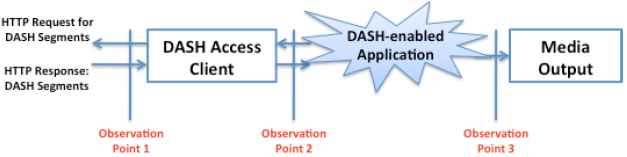
\includegraphics[width=\linewidth]{clientmodel}
	\caption{Model referencyjny klienta dla metryki DASH, źródło:~\cite{ISO-IEC-DASH}}
	\label{fig:clientmodel}
\end{figure}

Pierwszy punkt obserwacyjny znajduje się na styku połączenia sieciowego z komponentem aplikacji klienta odpowiedzialnym za zgłaszanie zapotrzebowania na dane i ich pobierania. W trakcie pracy tego komponentu monitorowane są:
\begin{itemize}
\item połączenia TCP - docelowy adres IP, czas rozpoczęcia, trwania i zakończenia połączenia,
\item sekwencja przesłanych wiadomości HTTP - czas transmisji, zawartość, połączenie TCP związane z transmisją,
\item odpowiedzi HTTP - czas otrzymania, zawartość nagłówka.
\end{itemize}

Drugi z punktów obserwacyjnych znajduje się pomiędzy komponentem odpowiedzialnym za pobieranie danych, a komponentem przetwarzającym otrzymane dane. Przetwarzanie danych może polegać na ich demultipleksowaniu (audio/video) lub dekodowaniu. W tym punkcie obserwacyjnym zbierane są informacje na temat kodowanych danych takie jak:
\begin{itemize}
\item typ danych - video, audio, tekst, itd...,
\item czas dostarczenia danych,
\item czas dekodowania danych,
\item poziom zapełnienia bufora dla pobieranych danych,
\item numer identyfikacyjny elementu \textit{Representation} z którego dane pochodzą.
\end{itemize} 

Ostatni z punktów obserwacyjnych znajduje się pomiędzy komponentem przetwarzającym dane oraz komponentem, który prezentuje przetworzone dane użytkownikowi.
\begin{itemize}
\item typ danych,
\item czas prezentowania danych wynikający z metadanych pliku MPD,
\item czas rzeczywisty prezentowania danych (timestamp),
\item numer identyfikacyjny elementu \textit{Representation} z którego dane pochodzą.
\end{itemize}

Tabele przedstawiające dokładną specyfikację metryk można znaleźć w specyfikacji standardu DASH-MPEG (\cite{ISO-IEC-DASH}) w dodatku D.

\section{DASH profiles}
\label{sec:profile}

Standard DASH definiuje kilka różnych profili identyfikowanych poprzez URN\footnote{Uniform Resource Name - jednolity format nazewnictwa zasobów.} i dopuszcza możliwość zdefiniowania własnego profilu identyfikowalnego za pomocą URN lub URL. Pojęcie profilu DASH jest konceptualnie podobne do profilu RTP/RTCP (zob. \ref{sec:rtp}) - jest to zestaw parametrów określających transmisję. Profile DASH mogą definiować ograniczenia lub wymogi odnoszące się zarówno do danych multimedialnych jak i do struktury tych danych znajdującej się na serwerze. W przypadku danych multimedialnych profil może określać np: obsługiwane kodeki\footnote{urządzenie lub program, który potrafi przekształcić strumień danych. Służy do kodowania i dekodowania strumieni danych. Przykłady: MP3, H.263, MPEG-2.}, kontenery\footnote{kontenery multimedialne poza danymi zawierają metadane potrzebne do właściwego odtwarzania danych multimedialnych. Przykłady: AVI, OGG, MKV.} oraz rozdzielczość. Ograniczenia nałożone na strukturę danych dotyczą zawartości plików MPD: ilości reprezentacji (\textit{Representation}), czasu trwania i wielkości segmentów, dostępnych bitrate, itp. Poniżej opisane zostały dwa z sześciu profili zdefiniowanych przez standard DASH. Specyfikacje pozostałych profili można znaleźć w \cite{ISO-IEC-DASH}.

\subsection{On Demand profile}

Ten profil został stworzony w celu dostarczenia podstawowych funkcjonalności w modelach On Demand. Cechą charakterystyczną tego profilu jest wymóg, by każdy element \textit{Representation} dostarczał pojedynczy \textit{Segment} podzielny na wiele elementów \textit{Subsegment}. Początek każdego z elementów typu \textit{Subsegment} powinien stanowić \textit{Stream Access Point}. Oznacza to, że aplikacja klienta może bez przeszkód rozpocząć odtwarzanie danych multimedialnych od dowolnego wybranego elementu \textit{Subsegment}. Aplikacja klienta może wcześniej zostać zainicjalizowana metadanymi znajdującymi się w odpowiednim \textit{Initialization Segment} lub każdy z \textit{Media Segments} może posiadać własne dane inicjalizujące.

Profil narzuca również pewne ograniczenia dotyczące struktury danych multimedialnych. Plik MPD nie może ulegać aktualizacjom w trakcie strumieniowania (tak jak to ma miejsce w przypadku transmisji na żywo). Wszystkie elementy \textit{Representation} muszą posiadać swoje \textit{Base URL} oraz posiadać parameter \textit{subsegmentStartWithSAP} ustawiony na wartość true. Ponadto dla dowolnych dwóch elementów \textit{Representation} w tym samym \textit{Adaptation Set} żadne dwa elementy \textit{Segment} nie mogą na siebie zachodzić (pod względem czasu odtwarzania) jeżeli ich numery sekwencyjne są różne (paramter \textit{segmentAlignment} ustawiony na true).

Wprowadzenie powyższych ograniczeń pozwala na skalowalne i wydajne wykorzystanie serwerów HTTP oraz ułatwia przełączanie pomiędzy wersjami danych multimedialnych w trakcie strumieniowania.

\subsection{Live profile}

Profil Live przeznaczony jest do obsługi strumieniowania danych multimedialnych na żywo. Wymogiem profilu jest krótki czas trwania elementów typu \textit{Segment}, standard nie precyzuje jednak tego wymogu za pomocą mierzalnych wartości. Od długości elementów \textit{Segment} zależeć będzie opóźnienie z jakim aplikacje klienckie będą otrzymywać dane. Im dłuższy \textit{Segment}, tym dłużej będzie trwało zebranie danych, ich zakodowanie, a następnie przesłanie do klientów. 

Podobnie jak w przypadku profilu On Demand, profil Live nakłada ograniczenie, dzięki któremu przełączanie pomiędzy różnymi wersjami tych samych danych jest ułatwione (\textit{segmentAlignment}). Ponadto, każda reprezentacja musi zawierać jeden \textit{Initialization Segment} oraz co najmniej jeden \textit{Media Segment}. 

\section{Podsumowanie}

DASH oferuje bogatą funkcjonalność w zakresie strumieniowania danych multimedialnych. Może zostać wykorzystany zarówno w systemach On Demand jak i do transmisji na żywo. Jako standard nie definiuje żadnych algorytmów strumieniowania adaptacyjnego, ale opisuje środowisko w którym takie algorytmy znalazły zastosowanie. Stos protokołów, który wykorzystuje decyduje o jego zaletach i wadach. Wykorzystanie protokołu TCP może powodować spore opóźnienia w transmisji, co zmniejsza przydatność DASH przy transmisjach na żywo. Zastosowanie protokołu HTTP pozwala na łatwe wdrożenie implementacji opartych na DASH w infrastrukturach sieciowych.

Dalsza część pracy skupia się na zagadnieniach algorytmów strumieniowania adaptacyjnego, testach ich skuteczności oraz problematyce pomiarów warunków panujących w sieciach komputerowych. Pomiary wykonywane w trakcie działania aplikacji nie mogą wpływać na sie. Niesie to za sobą koniecznoć oparcia tych pomiarów na parametrach transmisji wykorzystywanych do pobierania niewielkich segmentów danych multimedialnych. 

